\section{Resultados y discusión}
En busca de caracterizar una ferrita mixta de Mn y Zn, se observó la transición de fase ferromagnética-paramagnética de la muestra. En primer lugar, se registraron seis periodos correspondientes a la magnetización \(M\) y el campo coercitivo \(H\), que describen el ciclo de histéresis del material. De los seis ciclos registrados para cada temperatura se realizó un promedio punto a punto, obteniendo los ciclos de histéresis presentados en \autoref{histeresis}.

\begin{figure}[H]
    \centering
    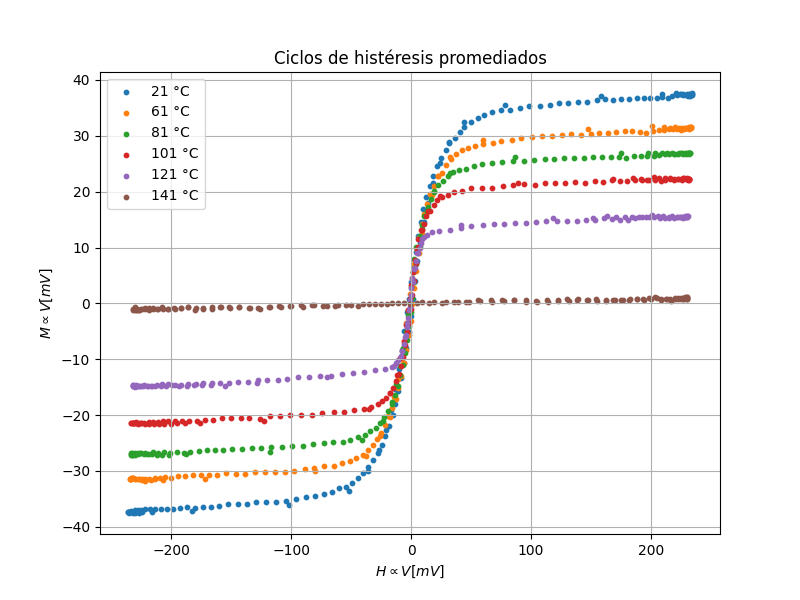
\includegraphics[width=0.8\textwidth]{Figuras 3/histeresis.png}
    \caption{Promedios de los ciclos de histéresis para las temperaturas registradas. En azul 21, en naranja 61, en verde 81, en rojo 101, en violeta 121 y en rosa 141 grados Celsius.}
    \label{histeresis}
\end{figure}

Puede observarse que, al aumentar la temperatura, el ciclo de histéresis se va cerrando, disminuyendo progresivamente la magnetización de saturación del material. A temperaturas cercanas a los 141 grados Celsius, el ciclo de histéresis practicamente desaparece, indicando que la muestra se encuentra próxima a la transición hacia la fase paramagnética.  

Tomando dos series de uno de los ciclos, se graficó la magnetización $M$ en función de la temperatura $T$, a fin de determinar la temperatura de Curie $T_c$ del material. Para esto, se utlizaron dos modelos: a temperaturas suficientemente bajas respecto a la de Curie, la magnetización del material se describe según la ley de Bloch \eqref{eq:Bloch}, donde se fijo el exponente $n$ en 1.5, valor característico de materiales ferromagnéticos. De los ajustes presentandos en la \autoref{bloch} se obtuvó una temperatura de Curie de $T_c = 166(1)$ grados Celsius, valor incompatible con la referencia de 135 grados Celsius ?. 

\begin{figure}[H]
\centering
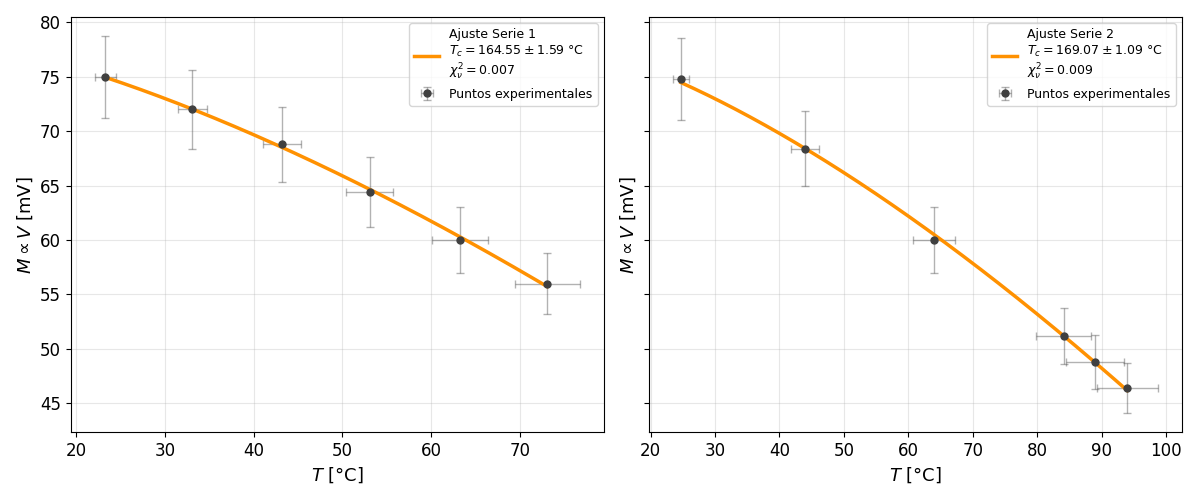
\includegraphics[width=0.9\textwidth]{Figuras 3/CurieBloch.png}
\caption{Ajustes de la magnetización en función de la temperatura mediante la ley de Bloch. En gris se presentan los datos experimentales, mientras que en amarillo se muestra el ajuste a la ley de Bloch. }
\label{bloch}
\end{figure}

Por otro lado, a temperaturas cercanas a la de Curie, la magnetización se describe mediante un comportamiento crítico derivado del modelo de Heisenberg, dado por la ecuación \eqref{eq:Heisenberg}. De los ajustes presentados en la \autoref{heisenberg} se obtuvo una temperatura de Curie de $T_c = 129.6(6)$ grados Celsius, valor también incompatible con la referencia. De este analisis se obtuvo además el valor del exponente crítico $\beta = 0.39(2)$, valor que si bien es cercano, no se corresponde con los valores típicos esperados para $\beta$, los cuales están entre 0.33 y 0.37.

\begin{figure}[H]
\centering
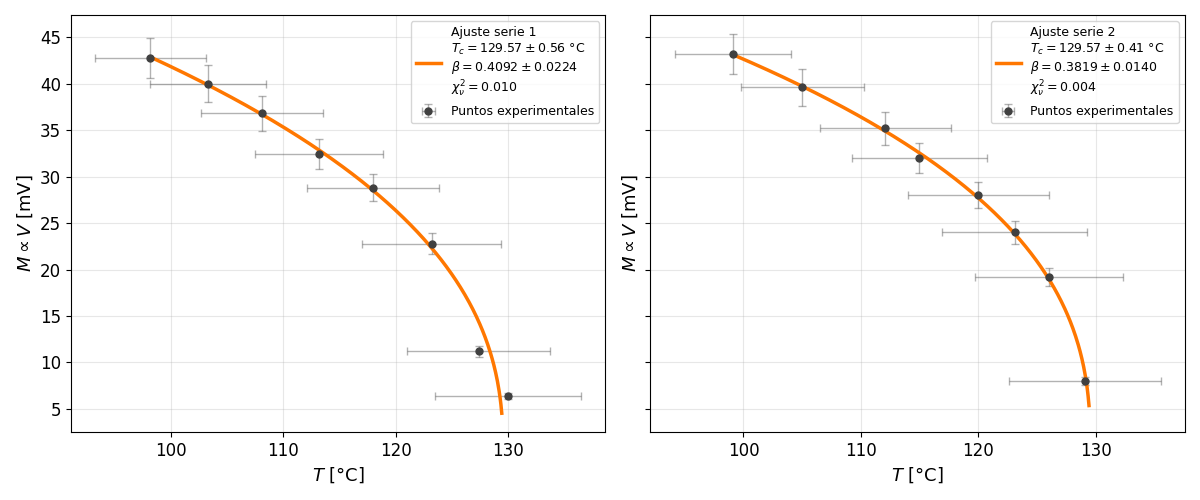
\includegraphics[width=0.9\textwidth]{Figuras 3/CurieHeisenberg.png}
\caption{Ajustes de la magnetización en función de la temperatura en las proximidades de la temperatura de Curie, utilizando el modelo de Heisenberg. En gris se presentan los datos experimentales, mientras que en amarillo se muestra el ajuste según el modelo de Heisenberg. }
\label{heisenberg}
\end{figure}

Finalmente, utilizando los valores de $T_c$ obtenidos tanto para Bloch como para Heisenberg, se confeccionó una recta de la $T_c$ en función de la fracción de Mn, utilizando la referencias teoricas para obtener el ratio de Mn y Zn en la muestra, como se presenta en \autoref{ratio}.  

\begin{figure}[H]
\centering
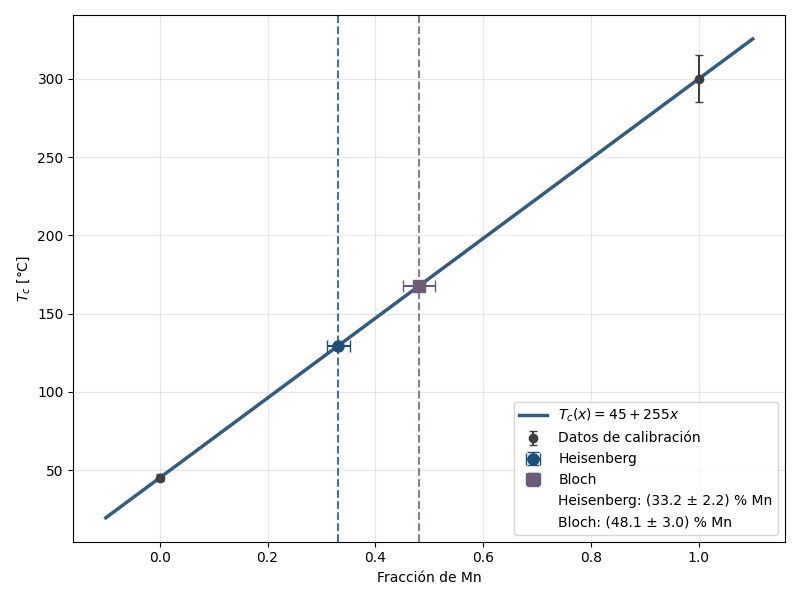
\includegraphics[width=0.75\textwidth]{Figuras 3/RatioZnMn.png}
\caption{Estimación de la fracción de Mn mediante la temperatura crítica obtenida con ambos modelos. En gris se representan los datos teoricos utilizados para la calibración, en celeste se muestra la recta de calibración, mientras que en violeta y azul se presentan las estimaciones de la fracción de Mn utilizando los valores de $T_c$ obtenidos con los modelos de Bloch y Heisenberg, respectivamente. }
\label{ratio}
\end{figure}

La interpolación sobre la recta de calibración permitió determinar la fracción de manganeso en la muestra, siendo de $x_H=33(2)\%$ para el modelo de Heisenberg y de $x_B=48(3)\%$ para el modelo de Bloch. Lo que indica una composición $Mn:Zn=0.49$ (?)
